\documentclass[a4paper,oneside,12pt]{article}
\usepackage{polyglossia}
\usepackage{microtype}
\setdefaultlanguage{english}
%\setotherlanguages{english}
\usepackage{fontspec}
\usepackage{amsmath}
\usepackage{amssymb}
\usepackage{amsfonts}
\usepackage{mathtools}
\usepackage{xltxtra}
\usepackage{xunicode}
\defaultfontfeatures{Mapping=tex-text}

\sloppy

%\usepackage[utf8]{inputenc}
%\usepackage[english,russian]{babel}
\usepackage{fancyhdr}
\usepackage[colorlinks=true,hidelinks]{hyperref}
\usepackage{ushort}
\usepackage{textcase}
\usepackage{tabularx}
\usepackage{colortbl}
\usepackage{graphicx}
\usepackage[x11names]{xcolor}
\usepackage[left=20mm,right=20mm,top=22mm,bottom=22mm]{geometry}
\setlength{\parindent}{0em}
\definecolor{dark}{RGB}{0,0,0}

\pagestyle{fancy}
\fancyhead{}
\fancyfoot{}
\fancyfoot[RO,RE] {\thepage}
\renewcommand{\headrulewidth}{0pt}
\renewcommand{\footrulewidth}{0pt}

\def\labelitemi  { \raisebox{0.1em} {$\scriptscriptstyle \blacksquare$} }
\def\labelitemii { \raisebox{0.1em} {$\scriptscriptstyle \Box        $} }
%\def\labelitemiii{ \raisebox{0.1em} {$\scriptscriptstyle $} }

\newcommand{\cvpart}[1]{%
\vspace{-0.9em}%
\section*{\Large\bfseries\MakeTextUppercase{#1}}%
\vspace{-1.7em}%
\rule{\linewidth}{0.3em}\\[-0.8em]%
}


\begin{document}

\begin{centering}
\begin{minipage}{0.70\linewidth}%
\vspace{-1.5em}{\Huge\bfseries Alexander Zheleznov}

~\\[-1.5em]

\hspace{1.9em}\begin{tabularx}{\linewidth}{ll}
{\it E-mail:}		& a.zheleznov@gmail.com\\
{\it Phone:}	        & +7\,(952)\,366-18-66 (mobile)\\
~\\[-1.0em] 
{\it Address:}	    & 196066\,~St.\,Petersburg\\
                    & ul.~Lensoveta kv.33\\
                    & Russia\\

~\\[-1.0em]
{\it Date of birth:}	& 12 June 1985\\
{\it Marital status:}& single\\
{\it Citizenship:}   & Russian Federation\\
{\it Languages spoken:}& English (advanced),\\ 
		       &Russian (native)\\
\end{tabularx}
\end{minipage}
\begin{minipage}{0.23\linewidth}%
\begin{flushright}
%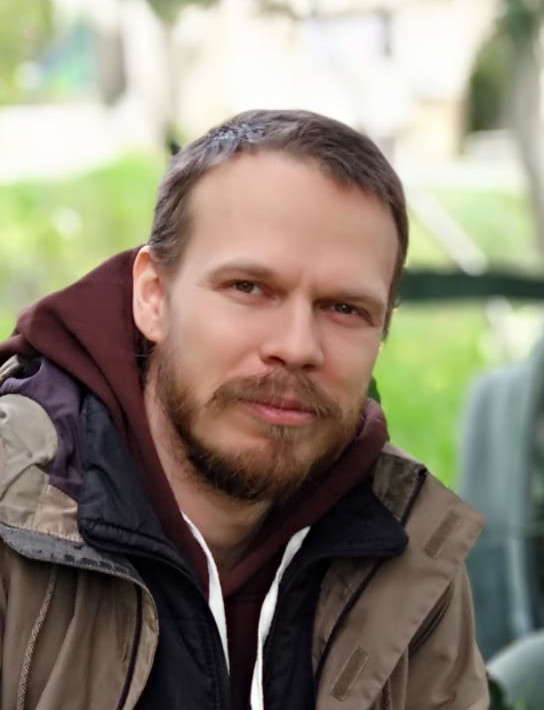
\includegraphics[width=35mm]{me.jpg}
{%
\setlength{\fboxsep}{0pt}%
\setlength{\fboxrule}{0pt}%
\fbox{
%    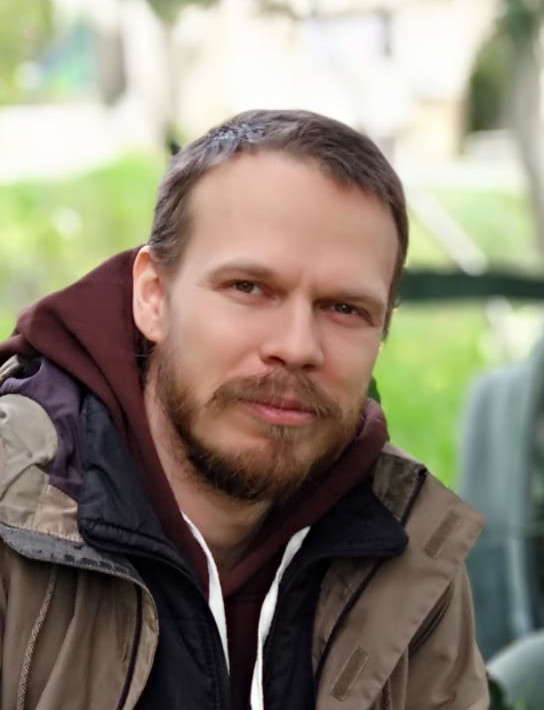
\includegraphics[width=35mm]{me.jpg}
}
}%
\end{flushright}
\end{minipage}
\end{centering}
~\\[1.5em]


\cvpart{Summary}
\begin{itemize}
\item 3 years of experience in UNIX programming environment (GNU/Linux).
\item Strong knowledge of C language (C99) and GNU toolchain.
\item Experience in development real-time applications under RTOS (ARINC--429, OS2000).
\item Experience in development of cross-platform applications (POSIX, libc).
\item Experience in development of unit tests.
    %\item Development of multithreaded applications (libpthread, OpenMP).
%\item Experience in Linux modules development.
%\item Version control systems (git, subversion).
\item Shell and lua scripting, software integration.
%\item Digital signal processing.
%\item Discrete math and algorithm design.
%\item Parallelization and vectorization techniques.
%\item Experience in project management.
\end{itemize}


\cvpart{Technical skills}
\begin{description}
\item[Operating systems:] Linux 2.6.x/3.x, MSDOS, Windows 98/XP/7.
\item[Programming languages:] C, C++, Lua. 
\item[Scripting languages:] Bash, awk, sed.   
\item[Developer tools:] GNU toolchain (GCC, gdb, make), git, (g)vim, qemu.
\item[Standards, technologies, libraries:] POSIX, ARINC--429, OpenMP, RapidIO, libc, libpthread, librt, GTK+, OpenGL, GLU. 
\item[Packaging:] Debian, Arch.
\item[Other skills:]  LaTeX, Octave/Matlab, gnuplot.
\end{description}


\cvpart{Employment}

\begin{tabularx}{\linewidth}{lX}
2012~-- to present:& CSPA Leninetz, Software Engineer.\\
\end{tabularx}

\pagebreak

\cvpart{Education}

\begin{tabularx}{\linewidth}{rX}
2014~-- to present:& Saint Petersburg State University (PhD student)\\
           faculty:& Applied Mathematics and Control Processes\\
        department:& Control of Medical and Biological Systems\\
                   & \\
      2008~-- 2013:& Saint Petersburg State University (graduate)\\
           faculty:& Applied Mathematics and Control Processes\\
        department:& Higher Mathematics\\
            Thesis:& ''\\ % TODO
            Degree:& Specialist's degree in Applied Mathematics and Information Technology
\end{tabularx}

~\\

\cvpart{Professional Experience}

{\bf
CSPA Leninetz, St.\,Petersburg, Russian Federation. Software Engineer. Full-time position.\\
July 2012~--- to present
}
Development of aircraft on board control systems.

\begin{itemize}
    \item Algorithm design and cross-platform(MIPS65, x86)  implementation for aricraft inertial navigation system.
\item Real-time inter process communication development for on-board control system (ARINC--429, RapidIO, OS2000, 0S3000).
%\item Cross-platform devdelopment for on board (MIPS64) and testing (x86) systems(C, GNU toolchain).
\item Developing unit tests for on board code (C, GNU toolchain, CppUtest).     
\item Porting on-board control system legacy code from MIPS64 to x86 (C, GNU toolchain).
\item Debugging and profiling of applications. (gdb, gprof).
%\item API design and writing documentation for interprocessor interaction framework (C99, doxygen).
%\item Software integration~--- developing test stand for on-board system certification (C, shell).
\end{itemize}

~\\[-1em]

\end{document}
